\section{Introdução}\label{sec:introducao}

% - Qual é a da coisa? (sintese c webaudio)
% - como a coisa funciona? 
%   - como um ou outro fez funcionar
%   - nosso jeito de funcionar

% -----------------------------------------------
 % http://www.charlie-roberts.com/pubs/Gibber_charles_roberts_icmc_2012.pdf


O processamento de sinais digitais de áudio em navegadores de rede, como por exemplo o Mozzilla Firefox, Google Chrome ou Apple Safari, é sumarizado por \cite{roberts_web_2013,wyse_viability_2014}. Utilizando a \emph{Web Audio API} \cite{w3c_web_2012} \emph{nós de áudio} podem ser concatenados em um grafo de DSP, como demonstrado na Figura \ref{fig:shime}. \cite{srikumar_tamming_2013} apresenta três instâncias de nós diferentes (\emph{OscilatorNode}, \emph{GainNode}, \emph{DestinationNode}), em sequência, para construir um simples sintetizador.

\begin{figure}[h]
\centering
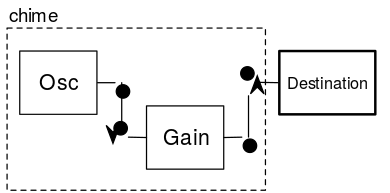
\includegraphics[scale=0.35]{chime.png}
\caption{Estrutura de síntese da API webaudio. \textbf{Fonte}: \cite{srikumar_tamming_2013}.}
\label{fig:shime}
\end{figure}

\subsection{GROOVE}

Este artigo envolve a utilização da tecnologia \emph{Web Audio} sob uma perspectiva histórica. Neste sentido, o trabalho de \cite{mathews_groove_1970}, GROOVE \footnote{\emph{Generated Real-time Operations On Voltage-controlled Equipment} \cite{serra_sound_2008,reynolds_resident_2012}.}, foi fundamental para a estruturação do \emph{Termpot}. 

Em um console de computador, um humano digita comandos, renderizados em som. O som, por sua vez, será percebido pela pessoa que controla a máquina, que fornecerá uma nova entrada de dados (através de novos comandos, ou dispositivos, como controles manuais). O sistema pessoa-máquina entra em um estado de \emph{feedback}, e o processo de síntese sonora considera questões performáticas. Um exemplo de música feita com o GROOVE, é \emph{The Expanding Universe} (1980) de Laurie Spiegel \cite{reynolds_resident_2012}\footnote{Disponível em \url{https://www.youtube.com/watch?v=dYUZmsfm4Ww}.}.

\section{Objetivos}

Descrever um programa \emph{web} desenvolvido com base no \emph{ScriptProcessorNode}, e estruturado segundo uma interpretação GROOVE.

%A Seção \ref{sec:trabalhos} deste artigo apresenta os frameworks supracitados e uma breve comparação entre eles.
%A Seção \ref{sec:termpot} apresenta a ferramenta proposta.
%A Seção \ref{sec:resultados} traz os resultados desta pesquisa e a Seção \ref{sec:conclusao} apresenta as conclusões do trabalho até o presente momento.

